% preamble
\documentclass{acm_proc_article-sp}

\usepackage{array}
\usepackage{xcolor}
\usepackage{graphicx}
\usepackage[final]{listings}
\usepackage{tikz}
\usepackage{verbatim}
\usepackage{cc}
\usepackage{syntax}
%\usepackage[hidelinks]{hyperref}
% lstlisting settings
\lstset{
    basicstyle=\ttfamily\small,
    breaklines=true,
    %language=scala,
    %numbers=left,
    numberstyle=\ttfamily\small,
    %showspaces=true,
    %showtabs=true,
    mathescape=true,
    %frame=single
}

% tikz settings/libraries
\usetikzlibrary{arrows}
\usetikzlibrary{shapes}
\usetikzlibrary{decorations.pathreplacing}
\usetikzlibrary{matrix}
\usetikzlibrary{positioning}
\usetikzlibrary{calc}
\usetikzlibrary{fit}

% version history styles
\tikzstyle{mytext} = [font=\scriptsize]
\tikzstyle{myhead} = [
    mytext,
    text centered,
    text width=3em,
    inner sep=2pt,
    rectangle,
    minimum height=1em,
    fill=red!20
]
\tikzstyle{mycode} = [
    mytext,
    text width=13em,
    inner sep=2pt,
    rectangle,
    draw
]
\tikzstyle{mycomm} = [
    mytext,
    text centered,
    text width=3em,
    inner sep=2pt,
    rectangle,
    rounded corners,
minimum height=1em
]
\tikzstyle{myyc} = [
    mycomm,
    fill=yellow!40
]
\tikzstyle{myrc} = [
    mycomm,
    fill=red!20
]

% flow diagram styles
\tikzstyle{mycond} = [
    mytext,
    text width=5em,
    inner sep=0pt,
    diamond,
    draw,
    fill=blue!20,
    text badly centered
]
\tikzstyle{myblock} = [
    mytext,
    text width=4em,
    inner sep=2pt,
    rectangle,
    draw,
    text centered,
    rounded corners
]
\tikzstyle{mygb} = [
    myblock,
    fill=green!20
]
\tikzstyle{myrb} = [
    myblock,
    fill=red!20
]
\tikzstyle{mycloud} = [
    mytext,
    draw, 
    ellipse,
    fill=red!20
]
\tikzstyle{myarrow} = [
    draw,
    -latex'
]

% defined commands
%\newcommand{\mytodo}[1]{{\color{red}\textbf{TODO:}}~#1}
\newcommand{\mytodo}[1]{%
    \par%
    \medskip%
    \noindent%
    %\fbox{%
    \parbox[s][1.4\height][c]{\columnwidth}{%
        {\color{red}\textbf{TODO:}}~#1%
    }%
    %}%
    \newline%
}

\newcommand{\myc}[3]{\ensuremath{#1\langle #2,#3\rangle}}
\newcommand{\myl}[1]{\ensuremath{#1}}
\newcommand{\myr}[1]{\ensuremath{\bar{#1}}}
\newcommand{\info}[1]{\color{blue}[#1]}
\newcommand{\gql}{GitQL}

\newcommand*{\ttf}{\fontfamily{cmvtt}\selectfont}

\setlength\extrarowheight{4pt}

\vfuzz2pt % allow overflow by 2 points
\hfuzz2pt % allow overflow by 2 points

%\renewcommand{\syntleft}{} 
%\renewcommand{\syntright}{}
%\renewcommand{\grammarlabel}[2]{\textit{#1}\hfill#2}


\title{Git Query Language and Variational Grep\\% 
    %CS~561 Fall~2015\\%
    %Final Project%
    \titlenote{%
        Does NOT produce the permission block, copyright information nor page numbering.
        For use with \lstinline|sig-alternate-05-2015.cls|.
        Supported by ACM.
    }%
}
\numberofauthors{2}
\author{
    \alignauthor
    %Deepthi Satish Kumar\\
    %\affaddr{College of Electrical Engineering and Computer Science}\\
    %\affaddr{Oregon State University}\\
    %\affaddr{Corvallis, OR}\\
    %\email{kumarde@oregonstate.edu}
    %\alignauthor
    %Spencer Hubbard\\
    %\affaddr{College of Electrical Engineering and Computer Science}\\
    %\affaddr{Oregon State University}\\
    %\affaddr{Corvallis, OR}\\
    %\email{hubbarsp@oregonstate.edu}
}

\begin{document}
    % front matter
    \maketitle
    
    % main matter
    \begin{abstract}
        %\input{abstract.tex}
    \end{abstract}
    \category{D.2.3}{Software Engineering}{Coding Tools and Techniques}%[Program editors]
    \terms{Design, Languages, Theory}
    \keywords{variation, version history, pattern matching, grep}
    
    
%    \section{Introduction}\label{sec:intro}
    %Introduction

%GQL is language to query the history of git repositories. Before going to the GQL, let us first see the need to query the history and how it is done till now is.

%\textbf{Why querying history is important}

One of the advantages of using version control systems (VCS) is that the users of a software repository can look at the evolution of the software. Users can see the changes that led to newer versions. These changes help users or programmers understand the workings of the current version because they can see what changed from the previous version. In the case of software bugs, users can quickly narrow down the part of code that caused it by identifying what changed between the version that worked correctly and the current version. Hence, the history of software plays a vital role in its maintenance. 


The history is important even during the development phase. A VCS makes it easier for the developers to try different implementations and choose one among them. This is either done by having a different implementation in a separate branch or by reverting to a previous version in the same branch in the case the latest implementation did not work. Querying even a shorter history helps the programmer to look at the changes she made and compare them.

Git, which is a distributed version control system has gained immense popularity over the last decade. A 2015 survey by Stackoverflow shows that 69.3$\%$ of the developers prefer git over other version control systems. Github ~\cite{github} which is a web-based version control system that uses git, hosts over 55 million projects. Hence, we looked at the history of projects that are version controlled by git.

%\textbf{Current commands and tools and why they are not sufficient}

Searching for a word or a sentence in a single file is an easy task supported by many tools.% and commands available. 
One can look for exact words or a pattern of words in which case a regular expression is used to specify the pattern. 
Grep is one such tool in Unix that can search a file using regular expression. 


In a file that is version controlled, searching involves looking into a specific version or all the versions of the file. To find a version that consists of a pattern, the user can create a script that runs grep on all the versions and returns	 the ones that contain the pattern. This brute-force approach is straightforward and easy to implement. However, it is not efficient when there are a huge number of versions.

An alternative is to use the commands provided by the VCS itself. Since these commands directly work on the internal representation, they are faster than the brute-force approach. In the case of git, commands like {\ttf git log}, {\ttf git diff}, and {\ttf git show} along with various options can be used to query the history. Some of the options allow users to search using regular expressions.

However, in cases where the users want to query the changes made to a particular part of the program, git commands do not suffice.
 
%\begin{comment}
%Consider a case where the user is looking for a specific change, that is, some string \textit{s} changed to \textit{t}.
%Git consists of commands that can be used to query what was added or removed in each version. 
%Such a command would return all the versions that added \textit{s} and all the versions that removed \textit{t} instead of just the version that replaced \textit{s} with \textit{t}.  Git also has commands that can track the changes made to a range of lines in the file. However, these are not accurate sometimes since the line numbers keep changing due to addition and deletion of lines.
%Most of these commands are complex and sometimes require external scripts as well.

%Consider a scenario where all the changes made to a function needs to be looked into for debugging purposes. A search for the function name will return all the versions that contain the function.  What we need in this case are all the versions that have some changes made to the function. Git log with the option -L searches the history of a range of lines specified by a start and an end. But this range will change when lines are added or deleted around the function, and therefore not all the changes are captured.
%\end{Comment}

Consider a scenario where two developers, Jen and Bob are working on a program that is version controlled by git, shown in listing~\ref{lst:ex1.1}. The program involves accessing user information from the database. The \ttf{elementOf} function parses a list of users and returns true if an arbitrary user exists otherwise false. This function is used before making expensive database access to retrieve any data about a user. 

\begin{lstlisting}[caption= Code snippet, label=lst:ex1.1, gobble=0, basicstyle=\ttfamily\small]
...
Boolean elementOf(ID userID)
{ 
 String userID = regexLookUp("*userID",this.userList);
  if(userID == "")
   return False;
  else
   return True;
}
...
User getUserInfo(ID userID)
{
 User user = Null;
 if(!elementOf(userID))
  throw new Exception("User not present");
 else
  user = getUserInfoFromDB(userID);
 return user;
}
...
\end{lstlisting}

Jen is working on a new feature and adds few methods to this program. Some of the new methods use \ttf{elementOf}. Listing ~\ref{lst:ex1.2} shows one of the new methods added by Jen.
Bob on the other hand is refactoring the existing code. He changes the method name \ttf{elementOf} to \ttf{isCurrentUser}. However, Bob renames it twice before arriving at this name. First, to \ttf{contains} and then to \ttf{present}, all of them committed to the repository. Listings ~\ref{lst:scr1}, ~\ref{lst:scr2} and ~\ref{lst:scr3} show the differences in each commit that renames the \ttf{elementOf} method.

\begin{lstlisting}[caption= Code snippet, label=lst:ex1.2, gobble=0, basicstyle=\ttfamily\small]
...
Link getUserlinks(ID userID1, ID userID2)
{
 User user1 = Null;
 User user2 = Null;
 if(!elementOf(userID1))
  throw new Exception("User %1 not present", userID1);
 if(!elementOf(userID2))
  throw new Exception("User %1 not present", userID2);
  
 user1 = getUserInfoFromDB(userID1);
 user2 = getUserInfoFromDB(userID2);
 return getlinks(user1,user2);
}
...
\end{lstlisting}

%\begin{figure}
%    \includegraphics[width=150mm]{scr1}
%    \caption{Renamed to \ttf{contains}}\label{fig:scr1}
%\end{figure}

\begin{lstlisting}[caption= Renamed to \ttf{contains}, label=lst:scr1, gobble=0, basicstyle=\ttfamily\small]
$\color{red}\texttt{-Boolean elementOf(ID userID)}$
$\color{green}\texttt{+Boolean contains(ID userID)}$
{
	String userID = regexLookUp("*userID",this.userList)
	if(userID == "")
$\color{blue}\texttt{@@ -19,7 +19,7 @@}$ Boolean elementOf(ID userID)
User getUserInfo(ID userID)
{
	User user = Null;
$\color{red}\texttt{-	if(!elementOf(userID))}$
$\color{green}\texttt{+	if(!contains(userID))}$
		throw new Exception("User not present");
\end{lstlisting}

\begin{lstlisting}[caption= Renamed to \ttf{present}, label=lst:scr2, gobble=0, basicstyle=\ttfamily\small]
$\color{red}\texttt{-Boolean contains(ID userID)}$
$\color{green}\texttt{+Boolean present(ID userID)}$
{
	String userID = regexLookUp("*userID",this.userList)
	if(userID == "")
$\color{blue}\texttt{@@ -19,7 +19,7 @@}$ Boolean elementOf(ID userID)
User getUserInfo(ID userID)
{
	User user = Null;
$\color{red}\texttt{-	if(!contains(userID))}$
$\color{green}\texttt{+	if(!present(userID))}$
		throw new Exception("User not present");
\end{lstlisting}

\begin{lstlisting}[caption= Renamed to \ttf{isCurrentUser}, label=lst:scr3, gobble=0, basicstyle=\ttfamily\small]
$\color{red}\texttt{-Boolean present(ID userID)}$
$\color{green}\texttt{+Boolean isCurrentUser(ID userID)}$
{
	String userID = regexLookUp("*userID",this.userList)
	if(userID == "")
$\color{blue}\texttt{@@ -19,7 +19,7 @@}$ Boolean elementOf(ID userID)
User getUserInfo(ID userID)
{
	User user = Null;
$\color{red}\texttt{-	if(!present(userID))}$
$\color{green}\texttt{+	if(!isCurrentUser(userID))}$
		throw new Exception("User not present");
\end{lstlisting}

%\begin{figure}
%    \includegraphics[width=150mm]{scr2}
%    \caption{Renamed to \ttf{present}}\label{fig:scr2}
%\end{figure}
%\begin{figure}
%    \includegraphics[width=150mm]{scr3}%[width=\columnwidth]{scr3}
%    \caption{Renamed to \ttf{isCurrentUser}}\label{fig:scr3}
%\end{figure}

Both Jen and Bob are working on different branches. First, Bob merges his changes with the main branch. After Jen merges her changes, she finds out that the program does not compile successfully. The method \ttf{elementOf} no longer exists. There are three ways to identify the problem.
\begin{description}
\item[1] Look for the file that contained \ttf{elementOf} and then search through the file that has the same implementation as \ttf{elementOf}.
\item[2] Go through all the commits, made after Jen created the branch, one by one.
\item[3] Search for the commit that renamed the method using the command \ttf{git log -G`elementOf'}. 
\end{description}

Option 1 and 2 are quite tedious if the implementation is complex or if the number of commits are large, respectively. The command in option 3 returns the commits that has \ttf{elementOf} in the added or removed lines. It shows even the commit that added the function for the first time. By going through the commits returned by the command, Jen sees that it was renamed to \ttf{contains}. However, that is not the latest name of the method. Jen has to then search again using \ttf{git log -G`contains'} to know what \ttf{contains} was renamed to and so on until the latest name is known. This comparatively takes less time than the other two options but nonetheless, is tedious.

Hence there is a need for a language that is simple, and that enables users not just to look for patterns but also to look for changes in the history of software repositories.

%\textbf{Prominent feature of GQL: Choice Patterns. Illustrated with an example}

In GQL, users can query the history similar to grep by using regular expressions.
The important feature, however, is to query specific changes. This can be achieved using the ``Choice Patterns."  In a choice pattern, users can specify a pattern for the text in the previous version and another pattern for the text in the later version. Therefore, retrieving only the versions that made such changes. The user can also specify the text in one version and obtain the subsequent changes made to it.

In the above example scenario, in GQL, Jen would query using the choice pattern \chc[d]{\ttf{elementOf},\ttf{\$x}} and obtain all the subsequent changes made to \ttf{elementOf}. The changes will be bound to the variable \ttf{x}. Choice patterns are explained in detail in section \ref{sec:gitql}.

\mytodo{specify the structure of rest of the paper}


\begin{comment}
For example, consider a C program shown in the listing~\ref{lst:v1}. The program consists of two functions along with the other functions; \texttt{get_record} returns a record value from a string in a particular format specified by the global variable \texttt{format}, \texttt{show_record} returns a string in the same format from a record value.

 the pattern to find the version in which a function \textit{foo} was renamed to \textit{bar} is \textit{\chc {foo,bar}}. The syntax for choice pattern is {\chc {\textit{Pattern-before}, \textit{Pattern-after}}}. The character {\dimMeta} is called the dimension which is explained in further sections.

\begin{lstlisting}[caption= C program that formats a record, label=lst:v1, gobble=0, basicstyle=\ttfamily\small]
#include <formatrecord.h>

char format[10] = "NAME:VALUE";

Record get_record(char[] string)
{ return formatter(string,format);}

...
...

char* show_record(Struct Record r)
{ return formatter(r,format);}
\end{lstlisting}
Say, the global variable \texttt{format} was changed twice in subsequent commits by a diferent programmer. In the first commit, the programmer renames the variable from \texttt{format} to \texttt{default_format}. Consequently, renames all the occurrences of \texttt{format}.  In second commit, the programmer adds a new format by creating another variable \texttt{current_format} and propagates the change to the function \texttt{get_record} to accept strings in the newer format. The programmer, however, forgets to rename the variable in the function \texttt{show_record}. Both the versions are shown in the listings ~\ref{lst:v2} and ~\ref{lst:v3} respectively. 

\begin{lstlisting}[caption= Program after the first commit, label=lst:v2, gobble=0, basicstyle=\ttfamily\small]
#include <formatrecord.h>

char default_format[10] = "NAME:VALUE";

Record get_record(char[] string)
{ return formatter(string,default_format);}

...
...

char* show_record(Struct Record r)
{ return formatter(r,default_format);}
\end{lstlisting}

\begin{lstlisting}[caption= Program after the second commit , label=lst:v3, gobble=0, basicstyle=\ttfamily\small]
#include <formatrecord.h>

char default_format[10] = "NAME:VALUE";
char current_format[10] = "NAME:VALUE1,VALUE2";

Record get_record(char[] string)
{ return formatter(string,current_format);}

...
...

char* show_record(Struct Record r)
{ return formatter(r,default_format);}

\end{lstlisting}

Now, the function \texttt{get_record} uses \texttt{current_format} whereas the function \texttt{show_record} uses \texttt{default_format}. 


%The merged program in shown in the listing ~\ref{lst:v4}.

%\begin{lstlisting}[caption= The same C program modified in branch 2 , label=lst:v4, gobble=0, basicstyle=\ttfamily\small]
%#include <formatrecord.h>
%
%char default_format[10] = "NAME:VALUE";
%char current_format[10] = "NAME:VALUE1,VALUE2";
%
%Record get_record(char[] string)
%{ return formatter(string,current_format);}
%
%...
%...
%
%char* show_record(Struct Record r)
%{ return formatter(r,default_format);}
%
%\end{lstlisting}

The program now reads the string in the appropriate format but writes in the old format. The programmer who coded the initial version knows only about the variable \texttt{format}. But the current code has two different variable names and so the programmer now, to understand the changes, wants to view all the changes that were made to the variable. With current git commands, the programmer has to first identify the commit that changed the variable name from \texttt{format} and then look for the commit that changed \texttt{default_format}. In GQL, this can be easily queried using the choice pattern \chc[d]{\texttt{format},\texttt{\$x}}. \texttt{\$x} contains all the new names of \texttt{format}. \texttt{\$x} is a query variable and is explained in the later section.

\end{comment}

%In the case where only one of the patterns is known, the other can simply be a variable which then refers to the entire text that was changed to or from. The texts stored in these variables can simply be displayed or queried further.




%A change in a file that leads to a new version can be viewed as a variation of the original file. Each edit made sequentially will create a new variant. At any point in time, any of these variants can be used. In git, this corresponds to cherry picking or reverting to a particular version. 
%A variational file consists of all the variations encoded in constructs called ``choices". The variational file of a file that is version controlled is created by adding choices for every change that leads to a new version. 
%[Explain Dimensions, alternatives, selections, decision]


%The version history is modelled using the choice edit model for text editors.[Cite, Explain chain edits and branch edits]

\begin{comment}
Software development involves a lot of variations. From changes in the specification to changes in the source code, most of these changes are important and need to be tracked. As the software project evolves over the year, the number of such changes increase. Often, one will look into the history of the project to understand why certain changes were made, to know when and who made those changes or to look for specific changes. This involves querying the history of the software repository. \\
    The paper presents a query language, \gql to search for changes in the history of a repository in Git. The aim is to provide a language that is expressive and intuitive which are lacking in the present command structure of Git.\\
    Using regular expression language to represent the patterns, \gql looks for specific variations in a file. The regular expression language is extended to add a construct to represent what we call a "Choice Pattern." Choice patterns are used to represent a specific change in the history. The entire version history of a file is represented as a variational string using the choice calculus and choice edit model.\\
    Git also provides commands that can be used to query using regular expression patterns. Therefore, we compared the performance of our language against the git commands and a simple script that runs grep command on all the versions of the file. Git commands work directly on its internal representation of the commit and therefore performs slightly faster. On the other hand, \gql performs better than the brute force of approach implemented in the script.
%The remainder of this paper has section 2 giving background on the choice calculus that is used to represent the change history of a file, Section 3 motivating our work with two example queries.
\end{comment}

         
%    \section{Background}\label{sec:back}
%    \subsection{The Choice Calculus}

To achieve the features of GQL, we represent the history of a repository using a formal language for variation called the choice calculus [Cite]. The choice calculus is a generic language that can be applied to an arbitrary object language. The choice calculus consists of \textit{choices} to denote variations. The syntax of a choice is {\chc {A,B,..}} where \textit{A},\textit{B} and so on are called the alternatives. The alternatives could be terms in the object language or choices themselves. Each of the alternatives in a choice leads to a different version. Therefore, a choice represents all possible variations of an expression in the object language from which one can be selected. Using the choice calculus representation, we get a simple tree model that allows to focus on the changes that lead to newer versions.
\mytodo{Cite paper, Eric's Ph.D. thesis, GTTSE tutorial}
Consider the example of two different implementations of a function \texttt{twice}.

\begin{lstlisting}
	int twice(int x) { return x+x; }
        
	int twice(int x) { return 2*x; }
\end{lstlisting}
        
We can capture the variation between the two implementations of the function \texttt{twice} in the choice expression.

\begin{lstlisting}
	int twice(int x) { $\chc{\texttt{x+x},\texttt{2*x}}$; }
\end{lstlisting}

Here, both the alternatives of the choice are terms in the object language, in this case, C.
A choice is bound to a dimension \textit{D}. Two choices can have same or different dimension names. To understand this better, in the above example, consider another implementation where the variable is named as \texttt{y}. Therefore, we now have one additional implementation of the function \texttt{twice}.

\begin{lstlisting}
	int twice(int y) { return y+y; }
        
	int twice(int y) { return 2*y; }
\end{lstlisting}        
	%int twice(int z){ return z+z}
        
	%int twice(int z){ return z*z}
        
The choice expression now has two dimensions, representing a variation in the variable name and function body respectively.%, therefore, capturing the fact that these are variations in two different aspects.

\begin{lstlisting}  
	int twice(int $\chc[B]{\texttt{x},\texttt{y}}$) { return $\chc[A]{\chc[B]{\texttt{x},\texttt{y}}\texttt{+}\chc[B]{\texttt{x},\texttt{y}},\texttt{2*}\chc[B]{\texttt{x},\texttt{y}}}$; } 
\end{lstlisting}


Two choices with dimension name \textit{B} are nested in the choice with dimension name \textit{A} thereby representing variations in multiple levels. This way, all the variants of a program in the object language can be represented using the choice calculus in one variational program.

From a variational program consisting of choices, a concrete program variant can be obtained by recursively selecting an alternative from each choice until all the choices are eliminated. The process of selecting an alternative from a choice is called \textit{selection}. A selection is a mapping from a dimension name to an alternative. The set of selections required to obtain a concrete program is called a \textit{decision}.

From the choice expression in the above example, to obtain the variant of \texttt{twice} which has \texttt{y} as the variable and implemented using \texttt{+}, we have to make two selections; one for the choice of variable names and the other for the choice of the function body. A selection is denoted by \textit{D}.l, \textit{D}.r where \textit{D} is the dimension name and l,r being abbreviation for `Left' and `Right' denotes the first and the second alternatives respectively.%1,2,..n are the indexes of the n alternatives that occur in the same order. 
The decision \{\textit{A}.l, \textit{B}.r\} will select the left alternative from the choice with dimension name \textit{A} and the right alternative from the choices with dimension name \textit{B} and produce the following concrete program in the object language.

\begin{lstlisting}
	int twice(int y) { return y+y; }
\end{lstlisting}
        
Here \textit{B}.R selects the second alternative from all the three choices that are named \textit{B}. The dimension names, therefore, synchronize the changes that are made in different places but are all part of the same variation. 

\subsection{The Choice Edit Model}

To represent the version history of a file using the choice calculus representation, we use the choice edit model[Cite] which is an application of the choice calculus representation. The choice edit model is a program edit model that can be used to understand and reason about the edits that a developer makes while editing a program. In the choice edit model, making an edit to a program is viewed as introducing variation into the program. Whenever a program part \textit{P} is changed to \textit{Q}, a choice between \textit{P} and \textit{Q} is introduced. Here, in a choice, the left alternative consists of the old value and the right alternative consists of the new value. %Consequently, selection can be expressed as \textit{D}.L and \textit{D}.R for left and right alternatives respectively. 
The object language, in this case, is simply a string of characters because we are capturing the textual edits and do not care if the program behavior changes or not.

Consider a C program \texttt{P} which consists of a function \texttt{f}. This is the first version of the function. %No changes have been made to it and therefore the variational program \textit{VP} is same as \textit{P}.

\begin{lstlisting} 
P = int f(int a)
    { int b; return a+b; }
\end{lstlisting}    
%VP = int f(int a)
%     {int b; return a+b;}


A programmer makes the following sequence of edits on \texttt{f}. After each edit, choices are created in the variational program.

\textbf{Edit 1:} Change the function argument to \texttt{c}. in the variation program \texttt{VP1}, a choice with dimension name, say \textit{A}, between \texttt{a} and \texttt{c} is introduced in all the places where the edit is made.

\begin{lstlisting}
P1 = int f(int c)
    { int b; return c+b; }
    
VP1 = int f(int $\chc[A]{\texttt{a},\texttt{c}}$)
     { int b; return $\chc[A]{\texttt{a},\texttt{c}}$+b; }
\end{lstlisting}

\textbf{Edit 2:} Assign the value 1 to the variable \texttt{b}. A choice with a different dimension name, say \textit{B}, between an empty string and ``\texttt{=1}" is introduced. This edit is an insert operation and therefore there is no old value. Similarly, for a delete operation there is no new value and therefore, the choice that represents a delete operation will have an empty string in the right alternative.

\begin{lstlisting}
P2 = int f(int c)
    { int b=1; return c+b; }
    
VP2 = int f(int $\chc[A]{\texttt{a},\texttt{c}}$)
     { int b$\chc[B]{,\texttt{=1}}$; return $\chc[A]{\texttt{a},\texttt{c}}$+b; }
\end{lstlisting}

\textbf{Edit 3:} Change the function argument again to \texttt{d}. A new choice with dimension name, say \textit{C}, is introduced. This edit is changing the string that has already been changed previously and therefore is nested in the right alternative of the choice with dimension name \textit{A}\\
. Such edits are called chain edits.

\begin{lstlisting}
P3 = int f(int d)
    { int b=1; return d+b; }
    
VP3 = int f(int $\chc[A]{\texttt{a},\chc[C]{\texttt{c},\texttt{d}}}$)
     { int b$\chc[B]{,\texttt{=1}}$; return $\chc[A]{\texttt{a},\chc[C]{\texttt{c},\texttt{d}}}$+b; }
\end{lstlisting}

For each edit operation, a new choice is introduced. To synchronize the edits made in different places, the choices are given the same dimension name. The variational program \texttt{VP3} now consists of the information on how the program was edited. It consists of all the edit operations that were made to the initial program \texttt{P}. The latest version can be obtained by selecting the right alternative from all the choices in \texttt{VP3}. The programmer can select any variant by making appropriate selections. For example, the decision \{\textit{A}.r,\textit{B}.l,\textit{C}.r\} will generate a variant that consists of Edit 1 and Edit 3 but not Edit 2 which, in terms of text editing, is called a selective undo. A selective undo feature allows the user to selectively choose which edits made to the program need to undone, instead of linearly undoing all the changes that were made one after the other. Similarly, a selective redo operation allows user to choose the edits that she wants to make again without having to linearly do all the edits. The program variant obtained after applying the decision \{\textit{A}.r,\textit{B}.l,\textit{C}.r\} is

\begin{lstlisting}
int f(int d)
{ int b; return d+b; }
\end{lstlisting}
    
%    \newpage
    
%    \section{Motivation}\label{sec:motiv}
%    Following are a few examples of queries and the results obtained using git commands and \gql.

\subsection{Query 1}
\textit{Find all the commits that affected a method foo.} \\
This command would involve a semantic search to identify the scope of a method block. However, neither git commands nor \gql search based on the syntax of the program. \\
Following are the two ways that can be used currently for this query.\\
\begin{description}
\item[1]. Use git grep to search for all the versions of find that contains the method foo and manually look at all the differences to identify if the method was changed.
\item[2]. Use git log with -L option that searches the history of a range of lines specified by a start and an end. But this range will change when lines are added or deleted around the method, and therefore every time a new commit affects the lines around the method; the query will change.
%The start and end parameters could also be a regex instead of the line number. \\ {\tt git log -L /foo/, /\}/:file.java}
\end{description}
When a method is added, a new choice is created between an empty string and the method. Further changes to this method will cause nested choices to be added in the right alternative of the initial choice. Therefore, the result of the above query is to find a choice and that introduced foo and then look for all the nested choices in the right alternative. \\
Following is the syntax of the queries in \gql.
\begin{description}
\item[] TO count number of commits that changed the method foo % \textit vs. \\
\begin{lstlisting}
 count (vgrep d$\langle$,*foo*$\rangle$ vs)
\end{lstlisting}
\item[] To show all the changes made to the method foo.
\begin{lstlisting}
 pretty (vgrep d$\langle$,*foo*$\rangle$ vs)
\end{lstlisting}
\item[] To further query the results
\begin{lstlisting}
vgrep pat from (vgrep d$\langle$,*foo*$\rangle$ vs)
\end{lstlisting}
\end{description}

\subsection{Query 2}
Were all the occurrences of a method name changed from 'foo' to 'bar'?

The distributive nature of git enables developers to work offline and then merge their commits. Sometimes this leads to merging conflicts that need to be resolved manually. Say, There were multiple branches created from the master at which point the method name was foo. Each branch renames the method differently, and while merging, one of the names is chosen, say 'bar'. To check if there are any occurrences of foo that was not merged correctly, the user would have to search for each of the different names. 

The following command in \gql can easily find all the occurrences that was not renamed from foo to bar.\\
\begin{lstlisting}
filter ("bar" `notIn` $ \$x $) from vgrep d$\langle$foo,$ \$x $ $\rangle$ vs
\end{lstlisting}

Here, the query first finds all the renames of foo and then filters the results based on whether the right alternative consists of bar or not. 
 










\begin{comment}
\subsection{Example 1}\label{ssec:ex1}
    
    Consider the following query - \\
    \textit{Find all the versions that consists of the function "foo"} \\
    There are two possible solutions to this query.
    \begin{description}
     \item[1] The following nested git command can be run. Such a command is not intuitive and requires a deeper understanding of the git command structure.
        \begin{lstlisting}
 git rev-list --all | GIT_PAGER=cat xargs git grep 'foo' 
        \end{lstlisting}
     \item[2] The brute force approach - a script to run grep on each version of the file by retrieving them one by one.
    \end{description}
    \subsection{Example 2}\label{ssec:ex2}
    Consider the following query - \\
    \textit{Find the commits that changed \tt{int} to \tt{long} }\\
    \\[2mm]
    The above query is to look for commit that changed the occurrence(s) of {\tt{int}} to {\tt{long}}.
    Using git commands, one can only find the commits that deleted {\tt{int}} and commits that added {\tt{long}} anywhere in the file. Both these results could point to different positions within the file.
    Figure ~\ref{fig:diff} is an example where the query should match the first change and not the other two.
    \begin{figure}
    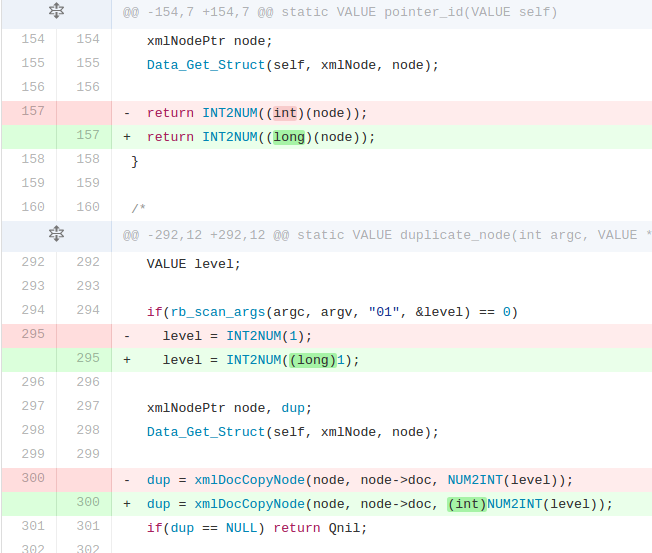
\includegraphics[width=\columnwidth]{diff}
    \caption{A commit that changed {\tt{int}} to \tt{long}}\label{fig:diff}
\end{figure}

gitQL is aimed at making such queries intuitive. It provides "choice pattern" constructs to specify the pattern for variations.
\end{comment}

\begin{comment}
Consider a scenario where a file consists of a function named foo. A branch is created from the main branch to add a different implementation of foo called baz while retaining foo. The user now decides to rename all the calls to foo to baz. 
Meanwhile, the function name foo its function calls were changed to bar in the main branch. 
Now, the newer implementation baz is better and tested thoroughly, and the developer decides to merge it. While merging the new implementation, of course, there is merge conflict and so the user resolves it by changing the function calls to bar to baz so as to retain the older function bar.

In the main branch, the function calls were changed from foo to bar and then again from bar to baz. 
At a later point, the software behaves funnily because some of the calls were still being made to bar. Therefore, the users want to look up all the places where the call to bar was not changed to baz. 

Using git commands, one will only find the versions that renamed foo to bar.  But we need all the subsequent changes in order to identify
\end{comment}
   
%    \section{Solution}\label{sec:sol}
%    A choice pattern is a pattern that is used to represent changes.
%    Choice Pattern : $$ d<P1,P2> $$
    
%A change consists of a state before and a state after. Therefore, to query a particular change, we specify a regular expression ($P1$) for the state before and a regular expression for the state after ($P2$).
%The 
    %\input{sol.tex}
    
%    \section{Results}\label{sec:res}
%    \input{res.tex}

%    \section{Related Work}\label{sec:rw}
%    \input{rw.tex}
    
%    \section{Conclusion}\label{sec:conc}
%    \input{conc.tex}
%    \newpage
    
    % back matter
    \bibliographystyle{abbrv}
    \bibliography{reference}
\end{document}
